\chapter{分子间作用力与溶剂}\label{ch:b1:intermolecular-forces-solvents}

壁虎沿窗玻璃向上爬，只靠一根脚趾挂在上面；
不靠胶水，也不靠吸力，只靠其趾垫分子与
玻璃分子之间的吸引。水分子比二氧化碳分子轻，却在
\qty{100}{\celsius} 沸腾，而二氧化碳在室温下是气体。
油漂浮在醋上，且与醋从不互溶；食盐
溶于水而不溶于汽油。这些现象并非由
分子内部的化学键决定，而是由它们之间弱得多的作用力决定。
本章对这些力进行分类，测量它们对沸点的影响，
并利用它们选择溶剂。

% ledger: bp:H2O (the hook's 100 degC)

\begin{recall}
第 1 册（十一年级）已介绍范德瓦耳斯力和氢键，
并解释了离子型固体如何通过解离与溶剂化而溶解。
偶极矩已在\cref{def:b1:lewis-resonance-vsepr:dipole}中定义，
极化率则在\cref{def:b1:periodicity:polarisability}中定义。
从物理学借用库仑定律：真空中两个电荷 $q_1$ 和 $q_2$ 相距
$r$ 处，相互吸引或排斥，其力的大小为 $|q_1q_2|/(4\pi
\varepsilon_0 r^2)$。
\end{recall}

\begin{omfigure}
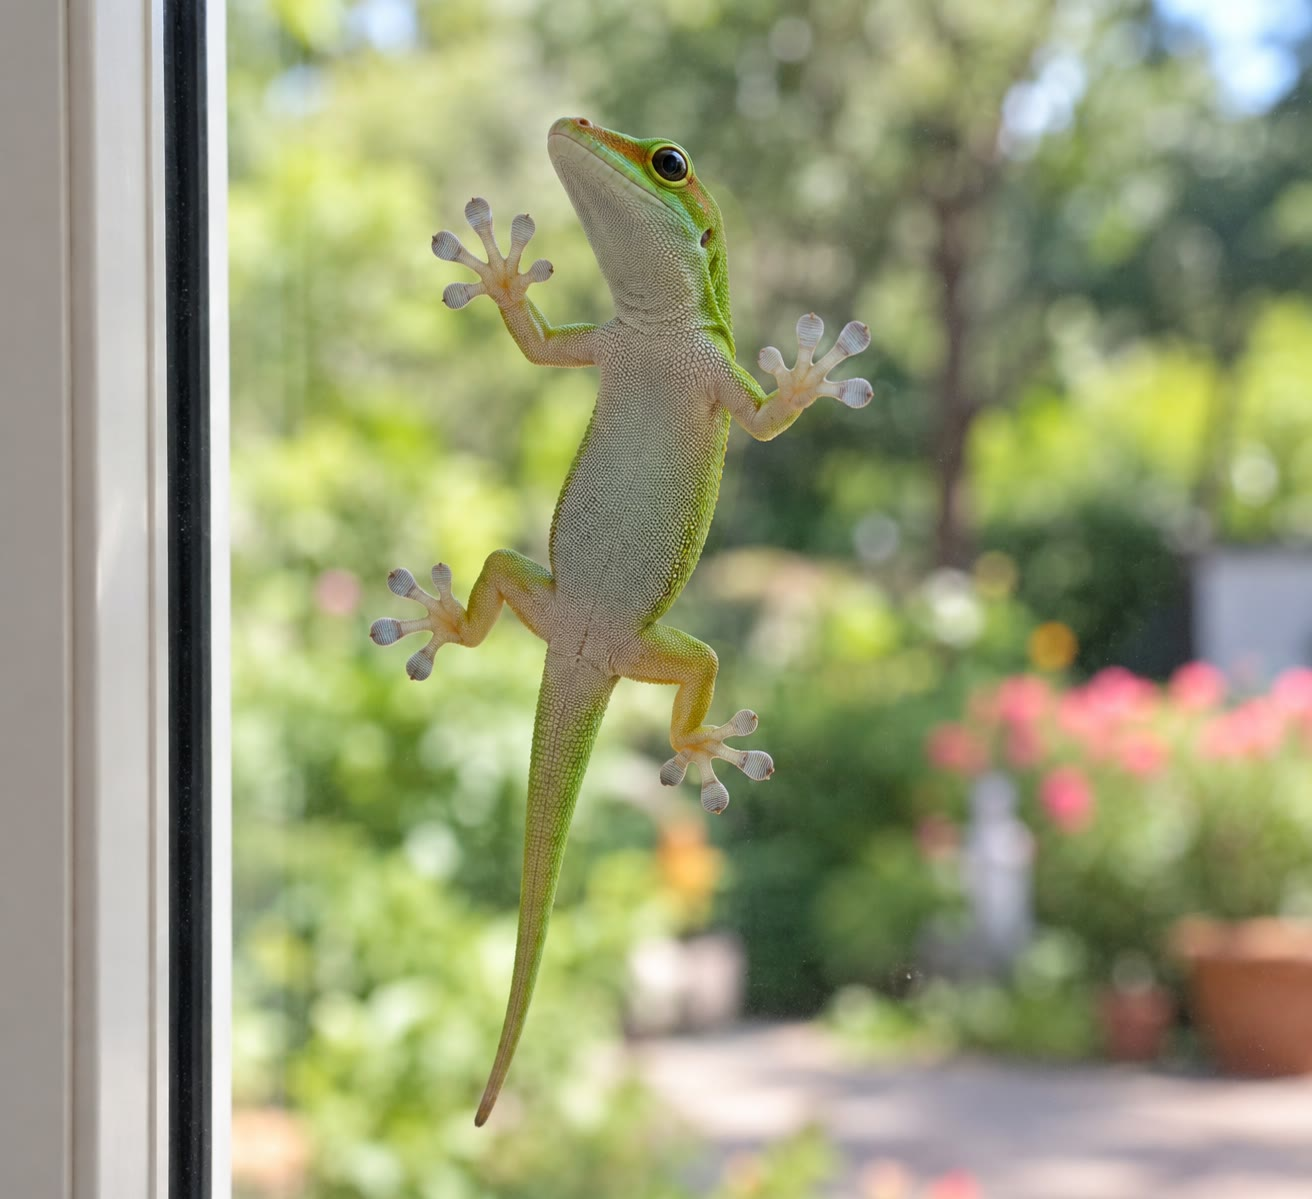
\includegraphics[width=0.52\linewidth]{images/book2/ai/b1-04-gecko.jpg}

{\small 窗玻璃上的壁虎。其趾垫上数以百万计的细毛
与玻璃极其接近，它们与玻璃分子之间微弱的吸引力
相加之和超过了壁虎的重力。}
\end{omfigure}

\section{范德瓦耳斯相互作用}

\begin{definition}[范德瓦耳斯相互作用]\label{def:b1:intermolecular-forces-solvents:vdw}
称\emph{范德瓦耳斯相互作用}\index{范德瓦耳斯相互作用}
为中性分子之间由其偶极相互作用产生的
吸引。可区分为三类：
\begin{itemize}
  \item \emph{葛生力}\index{葛生力}（或称
        取向作用），两个永久偶极之间的作用，
        它们倾向于首尾相接排列；
  \item \emph{德拜力}\index{德拜力}（或称
        诱导作用），永久偶极与
        它在可极化的邻近分子中诱导出的偶极之间的作用；
  \item \emph{色散力}\index{色散力}（或称
        色散作用），电子云的涨落在任意两个原子或分子中
        产生的瞬时偶极之间的作用，无论分子是否有极性，
        这些偶极相互诱导。
\end{itemize}
\end{definition}

\begin{omfigure}
\begin{tikzpicture}[font=\small, >={Stealth},
    mol/.style={draw=black!60, fill=#1, ellipse, minimum width=1.5cm, minimum height=0.8cm}]
  % Keesom
  \node[mol=omDef!20] (a) at (0,0) {}; \node[mol=omDef!20] (b) at (1.7,0) {};
  \node at (-0.45,0) {$\delta^-$}; \node at (0.45,0) {$\delta^+$};
  \node at (1.25,0) {$\delta^-$}; \node at (2.15,0) {$\delta^+$};
  \node[below, align=center] at (0.85,-0.65) {葛生力：\\两个永久偶极};
  % Debye
  \begin{scope}[xshift=4.6cm]
    \node[mol=omDef!20] at (0,0) {}; \node[mol=black!5, dashed] at (1.7,0) {};
    \node at (-0.45,0) {$\delta^-$}; \node at (0.45,0) {$\delta^+$};
    \node[omProp] at (1.25,0) {$\delta^-$}; \node[omProp] at (2.15,0) {$\delta^+$};
    \node[below, align=center] at (0.85,-0.65) {德拜力：\\永久与诱导偶极};
  \end{scope}
  % London
  \begin{scope}[xshift=9.2cm]
    \node[mol=black!5, dashed] at (0,0) {}; \node[mol=black!5, dashed] at (1.7,0) {};
    \node[omProp] at (-0.45,0) {$\delta^-$}; \node[omProp] at (0.45,0) {$\delta^+$};
    \node[omProp] at (1.25,0) {$\delta^-$}; \node[omProp] at (2.15,0) {$\delta^+$};
    \node[below, align=center] at (0.85,-0.65) {色散力：\\两个瞬时偶极};
  \end{scope}
\end{tikzpicture}

{\small 三种范德瓦耳斯相互作用示意。黑色部分电荷为
永久电荷（极性分子）；橙色为诱导或瞬时电荷。
每种情形下，相对的电荷符号相反，因此分子
相互吸引。}
\end{omfigure}

\begin{proposition}[强度与作用范围]\label{prop:b1:intermolecular-forces-solvents:distance-law}
对于相距为 $r$ 的两个分子，三种范德瓦耳斯
作用能量均按 $-1/r^6$ 变化：吸引只
在近邻之间才能感受到。其能量的数量级为每
摩尔几千焦，比共价键小约一百倍。色散项
随两个分子的极化率增大；它存在于
一切分子之间，通常是三者中最大的，
但对于小而强极性的分子则例外。
\end{proposition}
\admitted

\begin{example}[稀有气体与卤素]\label{ex:b1:intermolecular-forces-solvents:noble}
稀有气体的原子之间仅通过色散力相互吸引，
其强度随电子数增加而增大：氦的沸点为
\qty{-268.9}{\celsius}，氖为 \qty{-246.1}{\celsius}，氩为
\qty{-185.9}{\celsius}，氪为 \qty{-153.4}{\celsius}，氙为
\qty{-108.1}{\celsius}。同样，在室温下，二氟和
二氯为气体，二溴为液体（沸点为 \qty{58.8}{\celsius}），
二碘为固体。
% ledger: bp:He, bp:Ne, bp:Ar, bp:Kr, bp:Xe, bp:F2, bp:Cl2, bp:Br2, bp:I2
\end{example}

\begin{omfigure}
\begin{tikzpicture}
\begin{axis}[
  width=0.62\linewidth, height=5.4cm,
  xmin=0.5, xmax=10.5, ymin=-180, ymax=200,
  axis x line=bottom, axis y line=left,
  xlabel={碳原子数 $n$}, ylabel={沸点（\unit{\celsius}）},
  xtick={1,2,3,4,5,6,7,8,9,10}, ytick={-150,-100,-50,0,50,100,150},
  tick label style={font=\small}, label style={font=\small}]
\addplot[omDef, thick, mark=*, mark size=1.5pt] table[x=n, y=bp_C] {figdata/out/bachelor-1-hydride-boiling-points-alkanes.dat};
\end{axis}
\end{tikzpicture}

{\small 直链烷烃 \ce{C_nH_{2n+2}} 的沸点，从甲烷到
癸烷。每增加一个 \ce{CH2}，就增加电子数与接触面积，因而
色散力增强；沸点的增量缓慢减小，即从起始的约
\qty{75}{\celsius} 减至癸烷的 \qty{25}{\celsius}。}
\end{omfigure}

\section{氢键}

\begin{definition}[氢键]\label{def:b1:intermolecular-forces-solvents:hbond}
称\emph{氢键}\index{氢键}为一种吸引作用，
即 $\ce{X-H}\cdots\ce{Y}$ 中氢原子与一个体积小、电负性很强的
原子 X（\ce{N}、\ce{O} 或 \ce{F}）键合，与另一电负性较强的原子 Y 的孤电子对
相互作用。携带 \ce{X-H} 的分子是氢键供体，携带 Y 的
分子是氢键受体。其能量为 10
至 \qty{40}{kJ/mol}，介于范德华相互作用与共价键之间；
三个原子 \ce{X}、\ce{H}、\ce{Y} 近似共线。
\end{definition}

\begin{remark}[为何选 N、O 和 F]\label{rem:b1:intermolecular-forces-solvents:why}
电负性很强的 X 使氢带有较大的部分正电荷，
而氢无内层电子、体积极小，因而 Y 的
孤电子对可以非常靠近它。两个条件缺一不可：
\ce{C-H} 键极性不够强，\ce{S-H} 和 \ce{Cl-H} 键
所涉原子体积过大、电负性过弱，
难以形成强氢键。
\end{remark}

\begin{omfigure}
\begin{tikzpicture}[font=\small]
  % water network
  \foreach \n/\x/\y/\a in {1/0/0/0, 2/2.2/0.9/200, 3/0.2/-2.0/60, 4/-2.1/0.6/-30} {
    \begin{scope}[shift={(\x,\y)}, rotate=\a]
      \node[aO] (o\n) at (0,0) {};
      \node[aH] (h\n a) at (0.78,0.3) {};
      \node[aH] (h\n b) at (-0.2,-0.82) {};
      \begin{scope}[on background layer]
        \draw[bond] (o\n.center) -- (h\n a.center); \draw[bond] (o\n.center) -- (h\n b.center);
      \end{scope}
    \end{scope}
  }
  \draw[omThm, thick, densely dotted] (h1a) -- (o2);
  \draw[omThm, thick, densely dotted] (h1b) -- (o3);
  \draw[omThm, thick, densely dotted] (h4a) -- (o1);
  \node[below] at (0,-2.9) {水：每分子可给两个、受两个};
  % carboxylic acid dimer
  \begin{scope}[xshift=5.6cm, yshift=-0.6cm]
    \node (r1) at (-0.9,0) {R}; \node (c1) at (0,0) {C};
    \node (o1) at (0.6,0.85) {O}; \node (o2) at (0.6,-0.85) {O}; \node (h2) at (1.45,-0.85) {H};
    \node (c2) at (3.3,0) {C}; \node (r2) at (4.2,0) {R};
    \node (o3) at (2.7,0.85) {O}; \node (o4) at (2.7,-0.85) {O}; \node (h3) at (1.85,0.85) {H};
    \draw (r1) -- (c1) -- (o2) -- (h2) (c2) -- (r2) (c2) -- (o3) -- (h3);
    \draw[double, double distance=1.6pt] (c1) -- (o1); \draw[double, double distance=1.6pt] (c2) -- (o4);
    \draw[omThm, thick, densely dotted] (h2) -- (o4) (h3) -- (o1);
    \node[below] at (1.65,-2.3) {羧酸二聚体};
  \end{scope}
\end{tikzpicture}

{\small 氢键（红色虚线）。液态水中，每个分子至多参与
四个氢键；羧酸两两结合成环状二聚体，
由两个氢键维系。}
\end{omfigure}

\begin{proposition}[氢键使沸点升高]\label{prop:b1:intermolecular-forces-solvents:hbond-bp}
对第 15、16、17 族的氢化物，沸点从第 3 周期
增至第 5 周期而升高，遵循色散力的趋势；
而形成氢键的第 2 周期氢化物 \ce{NH3}、\ce{H2O} 和 \ce{HF}，
其沸点远高于该趋势的外推值。第 14 族氢化物
（\ce{CH4}、\ce{SiH4}、\ce{GeH4}）不形成氢键，
其沸点符合该趋势。
\end{proposition}

\begin{omfigure}
\begin{tikzpicture}
\begin{axis}[
  width=0.82\linewidth, height=6.6cm,
  xmin=1.5, xmax=5.6, ymin=-180, ymax=120,
  axis x line=bottom, axis y line=left,
  xlabel={周期}, ylabel={沸点（\unit{\celsius}）},
  xtick={2,3,4,5}, ytick={-150,-100,-50,0,50,100},
  tick label style={font=\small}, label style={font=\small},
  clip=false]
\addplot[black!60, thick, mark=square*, mark size=1.6pt] table[x=period, y=bp_C] {figdata/out/bachelor-1-hydride-boiling-points-g14.dat};
\addplot[omDef, thick, mark=*, mark size=1.6pt] table[x=period, y=bp_C] {figdata/out/bachelor-1-hydride-boiling-points-g15.dat};
\addplot[omThm, thick, mark=*, mark size=1.6pt] table[x=period, y=bp_C] {figdata/out/bachelor-1-hydride-boiling-points-g16.dat};
\addplot[omMeth, thick, mark=triangle*, mark size=2pt] table[x=period, y=bp_C] {figdata/out/bachelor-1-hydride-boiling-points-g17.dat};
\addplot[omThm, dashed] coordinates {(2,-79.3) (3,-60.3)};
\node[font=\small, anchor=west] at (axis cs:2.05,100) {水 \ce{H2O}};
\node[font=\small, anchor=west] at (axis cs:2.05,19.6) {氟化氢 \ce{HF}};
\node[font=\small, anchor=west] at (axis cs:2.05,-30) {氨 \ce{NH3}};
\node[font=\small, anchor=east] at (axis cs:1.96,-162) {甲烷 \ce{CH4}};
\node[font=\small, anchor=west] at (axis cs:4.05,-41.3) {硒化氢 \ce{H2Se}};
\node[font=\small, anchor=west] at (axis cs:5.05,-18.4) {锑化氢 \ce{SbH3}};
\node[font=\small, anchor=west] at (axis cs:5.05,-35.1) {碘化氢 \ce{HI}};
\node[font=\small, anchor=west] at (axis cs:4.05,-88.1) {锗烷 \ce{GeH4}};
\node[font=\small, omThm, anchor=north west] at (axis cs:2.05,-85) {外推};
\end{axis}
\end{tikzpicture}

{\small 氢化物的沸点：第 14 族（灰色方块）、第 15
族（蓝色）、第 16 族（红色）和第 17 族（绿色）。若水
按其较重同族（虚线）的趋势，沸点约为 \qty{-79}{\celsius}，
而氢键使其升高约 \qty{180}{\celsius}。}
% ledger: bp:CH4, bp:SiH4, bp:GeH4, bp:NH3, bp:PH3, bp:AsH3, bp:SbH3,
% bp:H2O, bp:H2S, bp:H2Se, bp:HF, bp:HCl, bp:HBr, bp:HI
\end{omfigure}

\begin{example}[乙醇及其同分异构体]\label{ex:b1:intermolecular-forces-solvents:isomers}
乙醇 \ce{CH3CH2OH} 与甲氧基甲烷 \ce{CH3OCH3} 具有相同的
化学式 \ce{C2H6O}，色散力几乎相同。乙醇，
其 \ce{O-H} 基团既是供体又是受体，沸点为
\qty{78.4}{\celsius}；甲氧基甲烷只能作受体，沸点为
\qty{-25.0}{\celsius}。
% ledger: bp:C2H5OH, bp:CH3OCH3
\end{example}

\section{溶剂}

\begin{definition}[相对介电常数]\label{def:b1:intermolecular-forces-solvents:permittivity}
在介质中，两电荷之间的库仑力被除以一个数
$\varepsilon_r \ge 1$，称为该介质的\emph{相对介电常数}\index{相对介电常数}
（或介电常数）：
\[
  F = \frac{|q_1 q_2|}{4\pi\varepsilon_0\varepsilon_r r^2} .
\]
极性分子构成的液体，其相对介电常数大，原因在于其分子会在电荷周围
定向排列并屏蔽电荷：水在 \qty{25}{\celsius} 时为 \num{78.4}，
己烷在 \qty{20}{\celsius} 时为 \num{1.89}。
% ledger: epsr:H2O, epsr:C6H14
\end{definition}

\begin{definition}[极性溶剂、质子性溶剂与非质子性溶剂]\label{def:b1:intermolecular-forces-solvents:solvent-classes}
\emph{极性溶剂}\index{极性溶剂}由偶极矩较大的分子组成，
其相对介电常数也较大（约在 15 以上）；
非极性溶剂则较小。\emph{质子性
溶剂}\index{质子性溶剂}的分子含有能形成氢键的氢原子
（\ce{O-H} 或 \ce{N-H}）；\emph{非质子性
溶剂}\index{非质子性溶剂}则不含此类氢原子。
\end{definition}

\begin{center}
\small
\begin{tabular}{lccll}
\hline
溶剂 & $\varepsilon_r$ & $\mu$ (D) & 极性 & 质子性 \\
\hline
水 & 78.4 & 1.86 & 极性 & 质子性 \\
甲醇 & 32.6 & 1.67 & 极性 & 质子性 \\
乙醇 & 24.3 & 1.52 & 极性 & 质子性 \\
乙腈，\ce{CH3CN} & 37.5 & 3.92 & 极性 & 非质子性 \\
丙酮 & 20.7 & 2.88 & 极性 & 非质子性 \\
二氯甲烷 & 9.08 & 1.62 & 弱极性 & 非质子性 \\
乙酸乙酯 & 6.02 & 1.78 & 弱极性 & 非质子性 \\
乙醚 & 4.34 & 1.15 & 弱极性 & 非质子性 \\
苯 & 2.28 & 0 & 非极性 & 非质子性 \\
己烷 & 1.89 & 0 & 非极性 & 非质子性 \\
\hline
\end{tabular}
\end{center}
% ledger: epsr:H2O, epsr:CH3OH, epsr:C2H5OH, epsr:CH3CN, epsr:CH3COCH3,
% epsr:CH2Cl2, epsr:EtOAc, epsr:Et2O, epsr:C6H6, epsr:C6H14, dip:H2O,
% dip:CH3OH, dip:C2H5OH, dip:CH3CN, dip:CH3COCH3, dip:CH2Cl2, dip:EtOAc,
% dip:Et2O, dip:C6H6 (relative permittivities at 20 or 25 degC; dipole
% moments of the gas-phase molecules; hexane has no dipole by symmetry)

\begin{definition}[溶剂化、电离能力与解离能力]\label{def:b1:intermolecular-forces-solvents:dissolution}
溶质粒子的\emph{溶剂化}\index{溶剂化}是指其被溶剂分子包围，
溶剂分子通过分子间作用力定向排列并与之结合
（在水中称为水合）。溶剂的\emph{电离能力}\index{电离能力}是指其能使溶质中的
极性共价键转变为离子对的能力，这是偶极矩较大的
极性溶剂所具有的性质；溶剂的\emph{解离能力}\index{解离能力}是指其
使离子对中的离子相互分离的能力，
这一能力以其
相对介电常数来衡量。
\end{definition}

\begin{proposition}[分三步溶解]\label{prop:b1:intermolecular-forces-solvents:steps}
电解质在溶剂中的溶解可分为三步：
电离（以 \ce{HCl} 这类分子型溶质为例）、离子对的解离，
以及分离后的离子的溶剂化。若溶剂为极性（具有电离能力）、
相对介电常数高（具有解离能力），并且能够溶剂化两种离子——
阳离子借助其孤电子对，阴离子若为质子性溶剂则借助氢键——
则它能很好地溶解离子型或强极性的溶质。
水同时具备这三种条件。
\end{proposition}

\begin{example}[氯化氢在水中与在己烷中]\label{ex:b1:intermolecular-forces-solvents:hcl}
在水中，\ce{HCl} 完全电离并解离：
\ce{HCl(g) + H2O(l) -> H3O+(aq) + Cl-(aq)}；溶液能导电。在
己烷中（非极性、介电常数低），\ce{HCl} 以
分子形式溶解，溶液不导电。
\end{example}

\begin{omfigure}
\begin{tikzpicture}[font=\small]
  \node[aNa] (na) at (0,0) {};
  \node[font=\scriptsize, white] at (na) {\ce{Na+}};
  \foreach \a in {0,60,...,300} {
    \begin{scope}[shift={(\a:1.25)}, rotate=\a]
      \node[aO] (o) at (0,0) {};
      \node[aH] (ha) at (0.55,0.5) {}; \node[aH] (hb) at (0.55,-0.5) {};
      \begin{scope}[on background layer]
        \draw[bond] (o.center) -- (ha.center); \draw[bond] (o.center) -- (hb.center);
      \end{scope}
    \end{scope}
  }
  \node[below] at (0,-2.4) {阳离子：氧的孤电子对朝内};
  \begin{scope}[xshift=6.2cm]
    \node[aCl] (cl) at (0,0) {};
    \node[font=\scriptsize, white] at (cl) {\ce{Cl-}};
    \foreach \a in {0,60,...,300} {
      \begin{scope}[shift={(\a:1.55)}, rotate=\a]
        \node[aH] (h1) at (-0.62,0) {};
        \node[aO] (o) at (0,0) {};
        \node[aH] (h2) at (0.25,0.72) {};
        \begin{scope}[on background layer]
          \draw[bond] (o.center) -- (h1.center); \draw[bond] (o.center) -- (h2.center);
        \end{scope}
      \end{scope}
    }
    \node[below] at (0,-2.4) {阴离子：氢键朝内};
  \end{scope}
\end{tikzpicture}

{\small 氯化钠两种离子的水合（仅第一层，
画在平面内）。水以其负端（氧原子）朝向
阳离子，并以一个氢原子朝向阴离子。}
\end{omfigure}

\section{溶解度、互溶性与两亲分子}

\begin{proposition}[相似相溶]\label{prop:b1:intermolecular-forces-solvents:like}
当溶质与溶剂分子之间的相互作用与其所失去的相互作用相当时，溶质易溶于该溶剂：
极性或能形成离子的溶质溶于极性溶剂，
非极性溶质溶于非极性溶剂，
能形成氢键的溶质溶于质子性溶剂。
\end{proposition}

\begin{proof}[推理]
溶解过程破坏溶质–溶质与溶剂–溶剂之间的相互作用，
并形成溶质–溶剂之间的相互作用。若溶质为非极性而溶剂为水，
水分子失去氢键以为溶质腾出空间，只换回较弱的伦敦力，
因此溶解不利。若二者均为非极性，
所失去与所形成的伦敦力相当，
则混合因其带来的无序度增加而有利。
\end{proof}

\begin{definition}[互溶液体]\label{def:b1:intermolecular-forces-solvents:miscibility}
两种液体若能以任意比例混合成单一液相，则称二者为\emph{互溶的}\index{互溶的}；
否则二者分成两层，
密度较小的一层位于上层。
\end{definition}

\begin{example}[水与乙醇、水与己烷]\label{ex:b1:intermolecular-forces-solvents:miscible}
乙醇与水互溶：二者均为质子性极性物质，且乙醇
既能与水形成氢键，也能与自身形成氢键。己烷与水
不互溶。二碘是分子晶体，在水中几乎不溶，但
易溶于己烷或二氯甲烷：与此类溶剂一同振荡时，水溶液中的碘
转入有机层，其原理即为
液–液萃取（见\cref{ch:b1:lab-techniques-1}）。
\end{example}

\begin{omfigure}
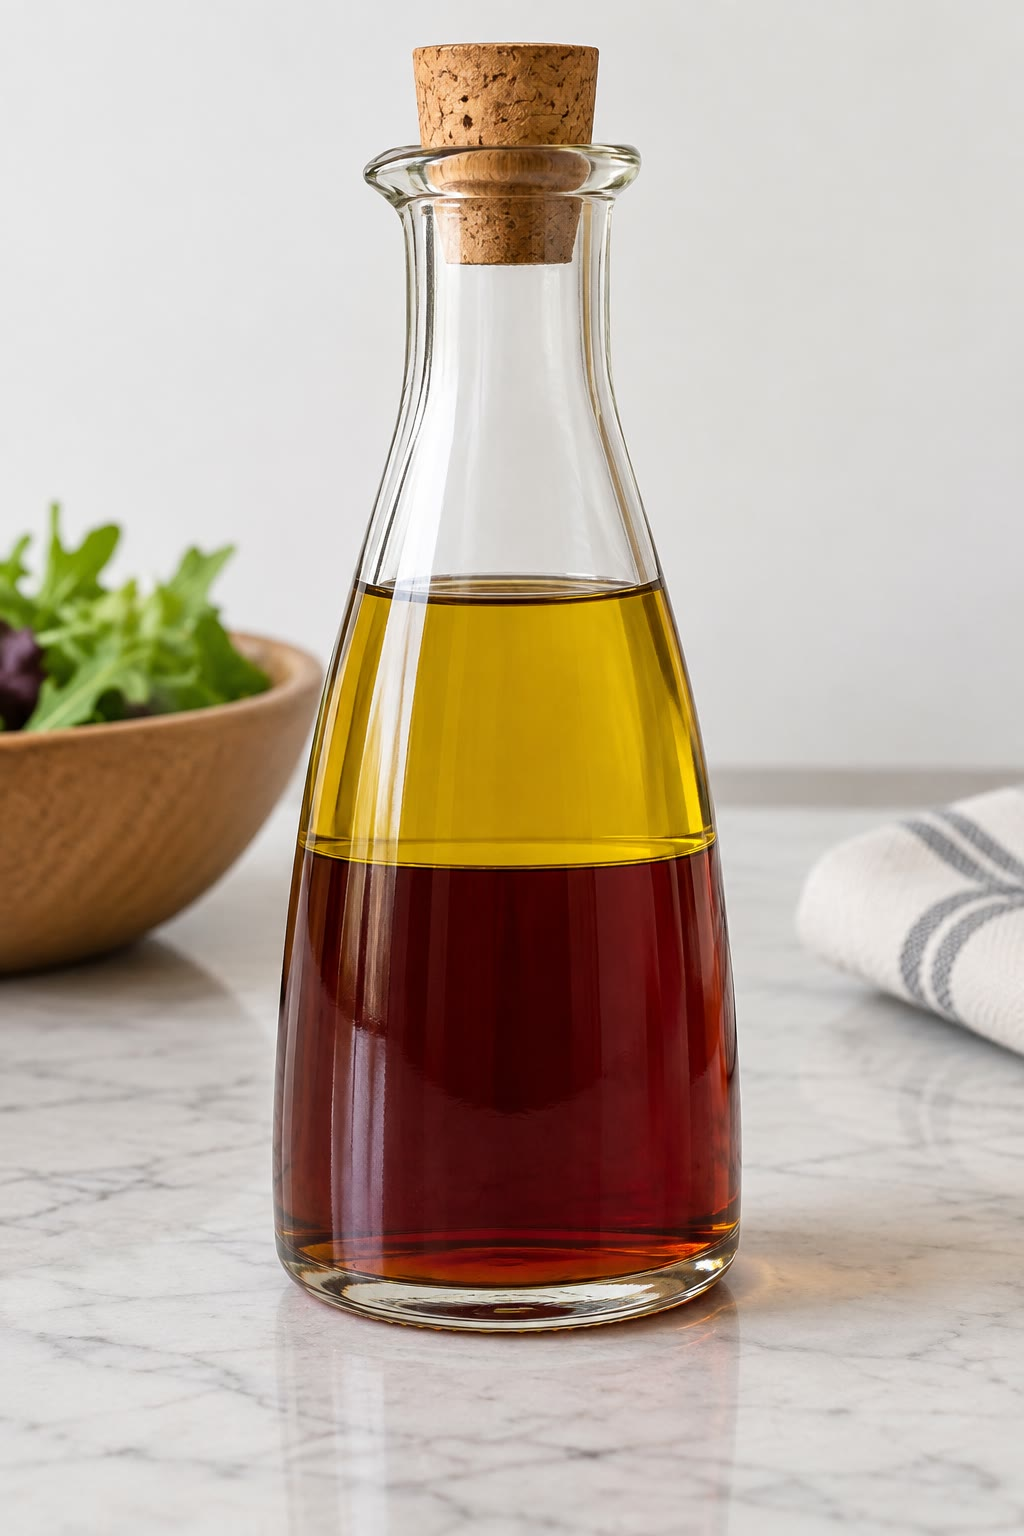
\includegraphics[width=0.2\linewidth]{images/book2/ai/b1-04-dressing.jpg}

{\small 静置的沙拉酱：橄榄油为非极性，漂浮于醋之上，
醋为水溶液，二者互不相溶。}
\end{omfigure}

\begin{definition}[亲水、疏水、两亲]\label{def:b1:intermolecular-forces-solvents:amphiphile}
当某基团与水发生有利的相互作用时，称其为\emph{亲水的}\index{亲水的}，
如离子基团或极性基团（\ce{-COO^-}、\ce{-OH}、
\ce{-SO3^-}）；不能时则为\emph{疏水的}\index{疏水的}（烃链）。
称分子为\emph{两亲的}\index{两亲的}，
当其同时带有亲水头部与疏水尾部时。
\end{definition}

\begin{example}[肥皂]\label{ex:b1:intermolecular-forces-solvents:soap}
十二酸钠，\ce{CH3(CH2)10COO- Na+}，为两亲分子。在
水的表面，其分子竖直排列，头部在水中，
尾部在空气中。在本体中，浓度超过一定值后，它们
聚集成球状——胶束——，尾部朝内，头部
朝外。非极性的油脂溶于胶束的疏水内核，
并被水带走。
\end{example}

\begin{omfigure}
\begin{tikzpicture}[font=\small]
  % interface
  \fill[omWater] (-3.2,-1.6) rectangle (-0.4,0);
  \draw[omDef!60] (-3.2,0) -- (-0.4,0);
  \node[anchor=south west] at (-3.2,0.95) {空气};
  \node[anchor=north west] at (-3.2,-1.2) {水};
  \foreach \x in {-2.9,-2.5,...,-0.6} {
    \fill[omThm] (\x,-0.12) circle (0.11);
    \draw[thick, black!70, decorate, decoration={zigzag, amplitude=1pt, segment length=3pt}] (\x,0) -- (\x,0.85);
  }
  % micelle
  \begin{scope}[xshift=3.2cm, yshift=-0.4cm]
    \fill[omWater] (-2,-1.6) rectangle (2,1.6);
    \foreach \a in {0,30,...,330} {
      \draw[thick, black!70, decorate, decoration={zigzag, amplitude=1pt, segment length=3pt}] (\a:0.25) -- (\a:1.0);
      \fill[omThm] (\a:1.12) circle (0.11);
    }
    \node[anchor=north] at (0,-1.65) {水中的胶束};
  \end{scope}
\end{tikzpicture}

{\small 两亲分子（红色亲水头部、锯齿形疏水
尾部）位于水表面，并聚集成胶束，按横截面绘制；
胶束在本科三年级分册中研究。}
\end{omfigure}

\begin{method}[选择溶剂]\label{met:b1:intermolecular-forces-solvents:choose}
为某溶质或某反应选择溶剂：
\begin{enumerate}
  \item 判断溶质类型：离子型、极性、能给出或接受
        氢键，或非极性；
  \item 选择同类溶剂（见\cref{prop:b1:intermolecular-forces-solvents:like}），
        若需使离子分离，则选用高介电常数的溶剂；
  \item 对于阴离子与分子之间的反应，优先选用极性
        非质子性溶剂，它能溶解该盐，而不以氢键束缚
        阴离子（见\cref{ch:b1:nucleophilic-substitution}）；
  \item 对于萃取，选择与原溶剂不互溶的溶剂，
        且溶质在其中的溶解度远大于在原溶剂中。
\end{enumerate}
\end{method}

\section{练习}

\begin{exercise}[$\star$]\label{exo:b1:intermolecular-forces-solvents:1}
写出液态氩、液态氯化氢、液态水、液态甲烷
与固态二碘中粒子间存在的相互作用，
并指出各体系中哪一种作用占主导。
\end{exercise}

\begin{exercise}[$\star$]\label{exo:b1:intermolecular-forces-solvents:2}
下列哪些物质的分子之间能形成氢键：
\ce{CH3OH}、\ce{CH3OCH3}、\ce{CH3NH2}、\ce{CH3F}、\ce{HF}、
\ce{CH4}？哪些只能接受来自其他分子的氢键？
\end{exercise}

\begin{exercise}[$\star$]\label{exo:b1:intermolecular-forces-solvents:3}
           利用溶剂表，将水、乙醇、丙酮、己烷、
           二氯甲烷和乙腈分为极性或非极性、质子性或非质子性。
\end{exercise}

\begin{exercise}[$\star$]\label{exo:b1:intermolecular-forces-solvents:4}
解释为什么二碘在己烷中比在水中溶解得多得多，
而氯化钠的情况则相反。
\end{exercise}

\begin{exercise}[$\star\star$]\label{exo:b1:intermolecular-forces-solvents:5}
甲醇的沸点为 \qty{64.7}{\celsius}，乙醇为 \qty{78.4}{\celsius}，
乙酸为 \qty{118.1}{\celsius}，二甲醚为
\qty{-25.0}{\celsius}。请解释这一顺序。
% ledger: bp:CH3OH, bp:C2H5OH, bp:CH3COOH, bp:CH3OCH3
\end{exercise}

\begin{exercise}[$\star\star$]\label{exo:b1:intermolecular-forces-solvents:6}
计算 \ce{Na+} 与 \ce{Cl-} 离子之间的库仑力，
二者相距 \qty{500}{pm}，在真空中（$\varepsilon_0 = \qty{8.854e-12}{F/m}$，
$e = \qty{1.602e-19}{C}$），再求在水中（$\varepsilon_r = 78.4$）及
在己烷中（$\varepsilon_r = 1.89$）时的值，并予以评论。
\end{exercise}

\begin{exercise}[$\star\star$]\label{exo:b1:intermolecular-forces-solvents:7}
丙酮与水以任意比例互溶，己烷与水
则不互溶。试从所断裂与所形成的相互作用角度加以解释。
\end{exercise}

\begin{exercise}[$\star\star$]\label{exo:b1:intermolecular-forces-solvents:8}
\ce{HCl} 的偶极矩为 \qty{1.09}{\debye}，其沸点为
\qty{-85.0}{\celsius}；\ce{HBr} 的偶极矩为 \qty{0.83}{\debye}，其沸点为
\qty{-66.4}{\celsius}。为何极性较小的分子沸点较高？
% ledger: dip:HCl, dip:HBr, bp:HCl, bp:HBr
\end{exercise}

\begin{exercise}[$\star\star$]\label{exo:b1:intermolecular-forces-solvents:9}
画出乙酸的环状二聚体。在苯溶液中，乙酸
的行为仿佛其摩尔质量约为 \qty{60}{g/mol} 的两倍，而在
水中则不然。试解释这两个事实。
\end{exercise}

\begin{exercise}[$\star\star\star$]\label{exo:b1:intermolecular-forces-solvents:10}
从解离与溶剂化的角度描述氯化钠在水中的溶解，
以及从电离、解离与溶剂化的角度描述氯化氢在水中的溶解。
为何氯化氢
在己烷中所得溶液不导电？
\end{exercise}

\begin{exercise}[$\star\star\star$]\label{exo:b1:intermolecular-forces-solvents:11}
由直链烷烃的沸点数据（戊烷
\qty{36.1}{\celsius}，癸烷 \qty{174.1}{\celsius}），
计算每个 \ce{CH2} 基团在 \ce{C5} 与 \ce{C10} 之间的平均沸点增量，
并估算十一烷的沸点。为何沿此系列
增量逐渐减小？
% ledger: bp:C5H12, bp:C10H22
\end{exercise}

\begin{exercise}[$\star\star\star$]\label{exo:b1:intermolecular-forces-solvents:12}
十二烷基硫酸钠，\ce{CH3(CH2)11OSO3^- Na+}，是一种洗涤剂。试指出
其亲水部分与疏水部分，画出它在水面及胶束中
的排布示意图，并解释它如何去除
织物上的油渍。
\end{exercise}

\section{周末问题：若水没有氢键}

\begin{problem}[{周末问题——稀有气体中的色散力，以及
烷烃中的色散力、溶剂的选择，以及若无氢键时水的沸点
将是多少}]
\label{pb:b1:intermolecular-forces-solvents:1}
在 \qty{1}{atm} 下的沸点（单位为 \unit{\celsius}）：\ce{He} $-268.9$，
\ce{Ne} $-246.1$，\ce{Ar} $-185.9$，\ce{Kr} $-153.4$，\ce{Xe} $-108.1$；
戊烷 36.1，己烷 68.8；\ce{CH4} $-161.5$，\ce{SiH4} $-112.0$，
\ce{GeH4} $-88.1$；\ce{NH3} $-33.4$，\ce{PH3} $-87.8$，\ce{AsH3} $-62.5$；
\ce{H2O} 100.0，\ce{H2S} $-60.3$，\ce{H2Se} $-41.3$；\ce{HF} 19.6，
\ce{HCl} $-85.0$，\ce{HBr} $-66.4$。
% ledger: bp:He, bp:Ne, bp:Ar, bp:Kr, bp:Xe, bp:C5H12, bp:C6H14, bp:CH4,
% bp:SiH4, bp:GeH4, bp:NH3, bp:PH3, bp:AsH3, bp:H2O, bp:H2S, bp:H2Se,
% bp:HF, bp:HCl, bp:HBr

\medskip
\noindent\textbf{第一部分——仅考虑色散力。}
\begin{enumerate}
  \item 哪一种相互作用使液态氩的原子保持在一起？
  \item 解释从氦到氙沸点升高的原因。
  \item 为何氦的沸点在所有物质中最低？
  \item 比较戊烷与己烷：每增加一个 \ce{CH2} 基团带来什么？
  \item 甲烷、硅烷与锗烷没有偶极矩。哪一种
        相互作用可以解释它们沸点的顺序？
  \item 为何甲烷中不可能形成氢键？
\end{enumerate}

\medskip
\noindent\textbf{第二部分——溶剂的选择。}
利用本章的溶剂表。
\begin{enumerate}[resume]
  \item 表中哪种溶剂最能溶解氯化钠，
        原因是什么？
  \item 在相同距离下，两个离子之间的吸引力在水中
        比在己烷中小多少倍？
  \item 阴离子 \ce{CN-} 与有机分子之间的反应，
        应在能溶解该盐而又不会通过氢键与
        该阴离子结合的溶剂中进行，请选出一种。
  \item 要从水溶液中萃取二碘，应选表中哪种溶剂，
        碘将最终位于哪一层？
  \item 解释为什么不能用乙醇进行该萃取。
  \item 乙醚虽为极性分子，却与水几乎不互溶。
        试提出一种解释。
\end{enumerate}

\medskip
\noindent\textbf{第三部分——其他氢化物。}
\begin{enumerate}[resume]
  \item 对第 17 族，计算从 \ce{HCl} 到
        \ce{HBr} 的沸点变化，并将同样的变化外推到第 2 周期。
  \item 将外推值与 \ce{HF} 的沸点作比较。
  \item 对第 15 族（\ce{PH3}、\ce{AsH3} 和
        \ce{NH3}）提出同样的两个问题。
  \item 对第 14 族，\ce{CH4} 位于由 \ce{SiH4} 和 \ce{GeH4} 外推所得直线的上方还是下方？
        为什么这一结果并不令人意外？
  \item 将 \ce{NH3}、\ce{HF} 和水的超出量排序。
  \item 统计 \ce{NH3}、\ce{HF} 和
        \ce{H2O} 每个分子能够给出和接受的氢键数目，并解释该排序。
\end{enumerate}

\medskip
\noindent\textbf{第四部分——不含氢键的水。}
\begin{enumerate}[resume]
  \item 为什么 \ce{H2S} 和 \ce{H2Se} 适合用于外推，
        而水本身不适合？
  \item 计算从 \ce{H2S} 到 \ce{H2Se} 的沸点变化。
  \item 写出通过这两点的直线方程，
        并以周期 $p$ 为变量。
  \item 推出在 $p = 2$ 时水应有的沸点。
  \item 氢键使水的沸点升高了多少？
  \item 得出结论：若水分子之间的吸引作用与 \ce{H2S} 分子相同，
        则水将在何温度下沸腾？
\end{enumerate}
\end{problem}
